\documentclass[aspectratio=169]{beamer}

\usepackage{amsmath,amssymb,amsfonts,amsthm}
\usepackage[T1]{fontenc}
\usepackage[utf8]{inputenc}
\usepackage[english]{babel}
\usepackage{hyperref}
\usepackage{lmodern}
\usepackage{comment}
\usepackage{xcolor}
\usepackage{graphicx,subcaption}
\usepackage{tikz,float}
\usetikzlibrary{positioning, fit}
\usepackage{tcolorbox}

\renewcommand{\epsilon}{\varepsilon}
\newcommand{\R}{\mathbb{R}}
\newcommand{\N}{\mathbb{N}}
\newcommand{\B}[2]{\mathcal{B}_{#1}\left(#2\right)}
\newcommand{\todo}[1]{{\color{red}#1}}

% Use Unipd as theme, with options:
% - pageofpages: define the separation symbol of the footer page of pages (e.g.: of, di, /, default: of)
% - logo: position another logo near the Unipd logo in the title page (e.g. department logo), passing the second logo path as option 
% Use the environment lastframe to add the endframe text
\usetheme[pageofpages=of]{Unipd}
\usefonttheme[onlymath]{serif}

\title{Random subsampling techniques for sea bass mortality prediction}
\author{Giovanni Gaio, Simone Moretti}
\date{\today}
\subtitle{}

\date{\today}

\begin{document}

\frame{\titlepage}

\begin{frame}
\frametitle{Overview}
\begin{itemize}
  \item Motivation: Identifying impactful SNPs in sea bass mortality
  \item Dataset: Genomic SNP data, mortality outcomes, and annotations
  \item Method: Subsampling techniques with XGBoost
  \item Results: Accuracy/F1 vs. subsampling rate
  \item Conclusion: Subsampling preserves predictive power
\end{itemize}
\end{frame}

\begin{frame}
\frametitle{SNPs and Sea Bass Mortality}
\begin{minipage}{0.45\textwidth}
  \textbf{Viral nervous necrosis} (\textbf{VNN}) is a highly spread disease among sealife.

  \vspace{2cm}

  We concentrate our study on a population of \textbf{sea basses} affected by VNN.
\end{minipage}

\begin{minipage}{0.45\textwidth}
    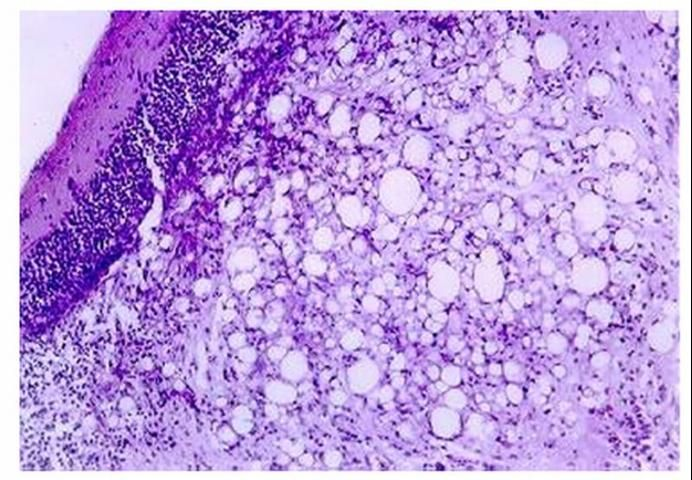
\includegraphics[width=0.6\linewidth]{figures/VNN.jpg}
    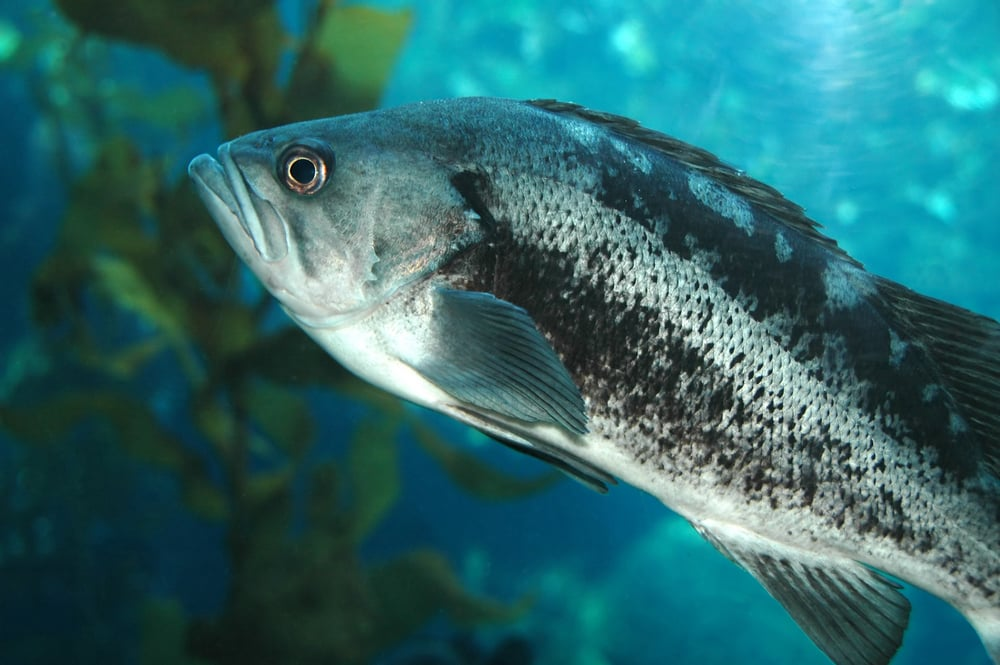
\includegraphics[width=0.6\linewidth]{figures/Black-Sea-Bass-303435837.jpg}
\end{minipage}
  
\end{frame}

\begin{frame}
\frametitle{Challenges with Genomic Data}
\begin{itemize}
  \item Each fish: over 6 million SNP positions.
  \item Sample size: only 990 sea bass individuals.
  \item Traditional models overfit due to data dimensionality.
\end{itemize}
\end{frame}

\begin{frame}
\frametitle{Machine Learning Approach}
\begin{itemize}
  \item Use XGBoost classifier for mortality prediction.
  \item Need to reduce feature space: apply subsampling.
  \item Evaluate performance on subsampled datasets.
\end{itemize}
\end{frame}

\begin{frame}
\frametitle{Pipeline Overview}
\begin{figure}[htb!]
    \centering
    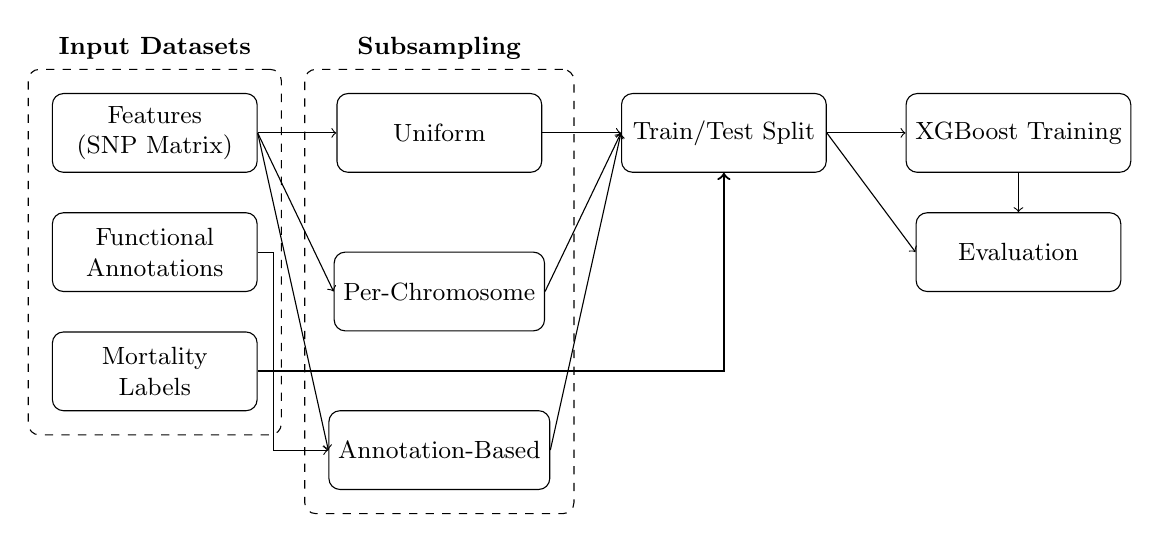
\begin{tikzpicture}[
        node distance=0.5cm and 0.1cm,
        every node/.style={font=\small},
        box/.style={draw, rectangle, rounded corners, minimum height=1cm, minimum width=2.6cm, align=center},
        group/.style={draw, rectangle, dashed, inner sep=0.3cm, rounded corners}
    ]

    \node[box] (features) {Features \\ (SNP Matrix)};
    \node[box, below=of features] (annotation) {Functional \\ Annotations};
    \node[box, below=of annotation] (mortality) {Mortality \\ Labels};

    \node[group, fit=(features)(mortality)(annotation), label=above:{\textbf{Input Datasets}}] (dataset_group) {};

    \node[box, right=1cm of features] (uniform) {Uniform};
    \node[box, below=1cm of uniform] (chr) {Per-Chromosome};
    \node[box, below=1cm of chr] (annot) {Annotation-Based};

    \node[group, fit=(uniform)(chr)(annot), label=above:{\textbf{Subsampling}}] (subsampling_group) {};

    \node[box, right=1cm of uniform] (split) {Train/Test Split};
    \node[box, right=1cm of split] (xgboost) {XGBoost Training};
    \node[box, below=of xgboost] (evaluate) {Evaluation};

    \draw[->] (features.east) -- ++(0.1,0) |- (uniform.west);
    \draw[->] (features.east) -- (chr.west);
    \draw[->] (features.east) -- (annot.west);

    \draw[->] (annotation.east) -- ++(0.2,0) |- (annot.west);

    \draw[->] (uniform.east) -- ++(0.1,0) |- (split.west);
    \draw[->] (chr.east) -- (split.west);
    \draw[->] (annot.east) -- (split.west);

    \draw[->, thick] (mortality.east) -| (split.south);

    \draw[->] (split.east) -- (xgboost.west);
    \draw[->] (split.east) -- (evaluate.west);
    \draw[->] (xgboost.south) -- (evaluate.north);

    \end{tikzpicture}
    \caption{Pipeline of the model training after subsampling of the data}
    \label{fig:pipeline}
\end{figure}
\end{frame}

\begin{frame}
\frametitle{SNP Dataset Structure}
\begin{itemize}
  \item 990 rows (fish), each with 6,072,853 SNP features.
  \item SNP values: 0 (no mutation), 1 (heterozygous), 2 (homozygous alt).
  \item Each fish is paired with a mortality label.
\end{itemize}
\end{frame}

\begin{frame}
\frametitle{Annotation Metadata}
\begin{itemize}
  \item Annotations include function: Promoter, Enhancer, Open Chromatin.
  \item Tissue number (0–25) indicates location-specific relevance.
\end{itemize}
\end{frame}

\begin{frame}
\frametitle{Uniform Subsampling}
\begin{itemize}
  \item Randomly sample a fixed proportion $p$ of all SNPs.
  \item Simple but may cause imbalance across chromosomes.
\end{itemize}
\end{frame}

\begin{frame}
\frametitle{Per-Chromosome Subsampling}
\begin{itemize}
  \item Ensures balanced representation from each chromosome.
  \item Randomly sample same number of SNPs per chromosome.
\end{itemize}
\end{frame}

\begin{frame}
\frametitle{Annotation-Based Subsampling}
\begin{itemize}
  \item Filter SNPs by biological annotation.
  \item Then apply uniform subsampling to relevant regions.
\end{itemize}
\end{frame}

\begin{frame}
\frametitle{Subsampling Strategy Comparison}
\begin{itemize}
  \item Trade-offs in simplicity, biological interpretability, and balance.
  \item Aim: maximize predictive power while reducing dimensionality.
\end{itemize}
\end{frame}

\begin{frame}
\frametitle{Control of Randomness}
\begin{itemize}
  \item XGBoost random seed fixed.
  \item Train-test split fixed
  \item Subsampling is the only random step.
\end{itemize}
\end{frame}

\section{Results}
\begin{frame}
\frametitle{Subsampling Ratios}
\begin{itemize}
    \item Subsampled with multiple $p$ values: log-spaced varying from the whole genome to few SNPs.
  \item Trained model for each combination of model and subsample rate.
  \item Multiple runs for each pair of parameters.
\end{itemize}
\end{frame}

\begin{frame}{Results: uniform subsampling}
\begin{figure}[H]
    \centering
    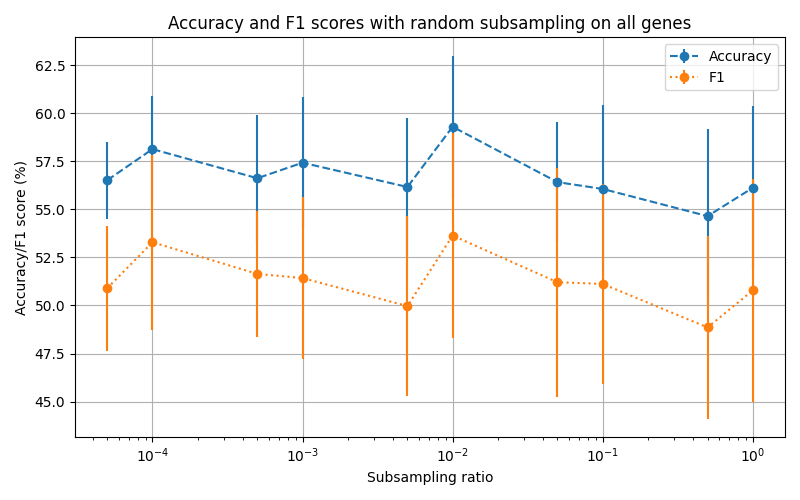
\includegraphics[height=0.5\textwidth]{../figures/subsample_plot.png}
    \caption{Plot of accuracy and F1 scores when subsampling uniformly on the whole genome.}
    \label{fig:res1a}
\end{figure}
\end{frame}

\begin{frame}{Results: observations}
\end{frame}

\begin{frame}{Results: uniform subsampling on each chromosome}
\begin{figure}[H]
    \centering
    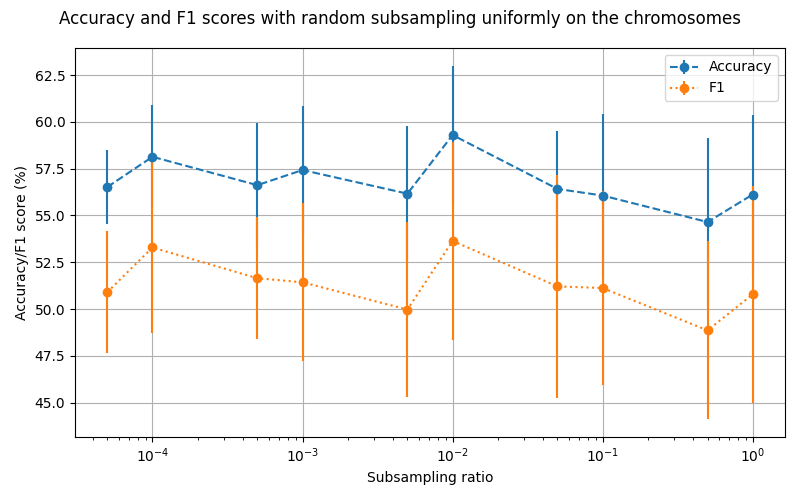
\includegraphics[height=0.5\textwidth]{../figures/uniform_sample_low_ratio.png}
    \caption{Plot of accuracy and F1 scores when subsampling uniformly on each chromosome.}
    \label{fig:res1b}
\end{figure}
\end{frame}

\begin{frame}{Results: observations}
\end{frame}

\begin{frame}{Results: annotated subsampling (function)}
\begin{figure}[H]
    \centering
    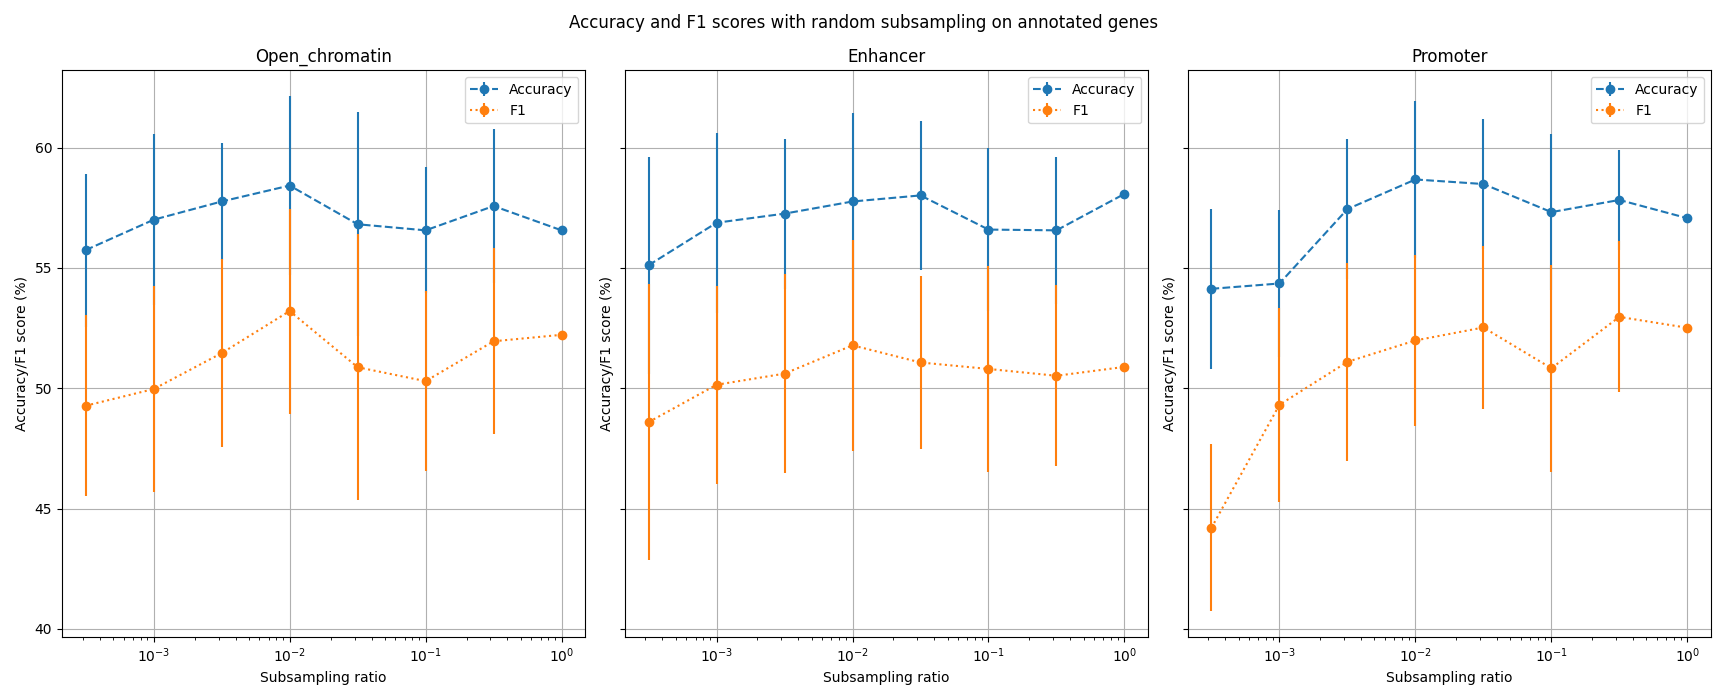
\includegraphics[width=\textwidth]{../figures/subsample_annotated.png}
    \caption{Plot of accuracy and F1 scores when subsampling uniformly on each chromosome.}
    \label{fig:res1a}
\end{figure}
\end{frame}

\begin{frame}{Results: annotated subsampling (tissue number)}
\begin{figure}[H]
    \centering
    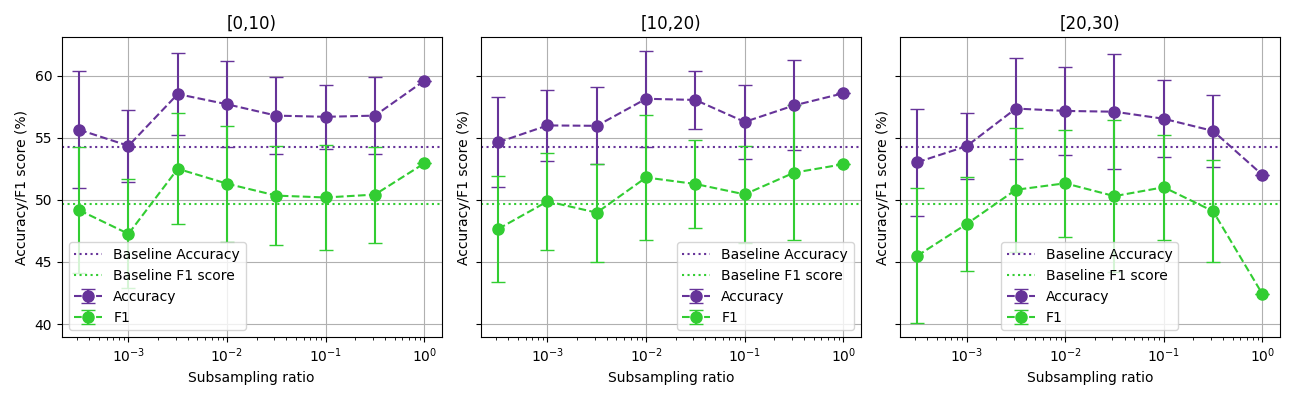
\includegraphics[width=\textwidth]{../figures/subsample_ntissue.png}
    \caption{Plot of accuracy and F1 scores when subsampling uniformly on each chromosome.}
    \label{fig:res2b}
\end{figure}
\end{frame}

\begin{frame}{Results: observations}
\end{frame}

\section{Conclusions}
\begin{frame}
\frametitle{Conclusions}
\begin{minipage}{0.60\textwidth}
\begin{itemize}
  \item Random SNP subsampling retains model effectiveness.
  \item No strong trend between rate and accuracy (outside extremes): this may be good.
  % \item Enables faster, scalable experimentation for genomic prediction.
  \item There doesn't seem to be specific regions of the genome containing the information determining the disease effects.
\end{itemize}
\end{minipage}
\begin{minipage}{0.35\textwidth}
    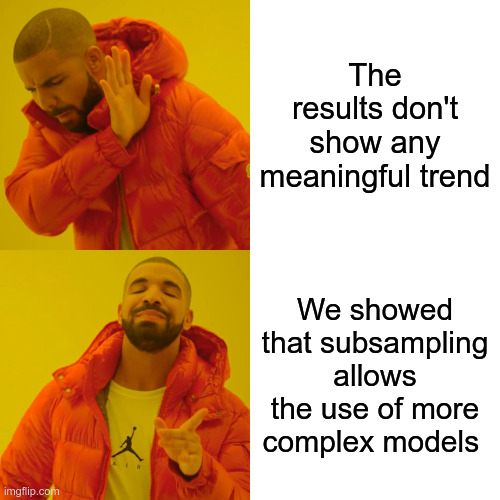
\includegraphics[width=0.99\textwidth]{memes/drake_results.jpg}
\end{minipage}
\end{frame}

\begin{frame}{End}
\centering
\Huge Thank You
\end{frame}

\end{document}
